\documentclass[main]{subfiles}

\begin{document}


\section{Concurrency}
In the introductory chapter, we saw how several threads accessing the same objects can lead to incorrect or undesirable executions and dubbed such cases \textbf{data races}. In this chapter, we'll first define the term mutual exclusion and the properties that can be associated with mutual exclusion. We'll then implement mutual exclusion as locks.\\
To widen our understanding of mutual exclusion implementations, we'll have a look at some of the more high-level synchronization primitives such as semaphores and barriers. Implementing what we've learned, we'll then look at different strategies of implementing concurrent data structures, moving from locked structures to lock-free structures. After having seen some of the challenges of lock-free programming, we'll finally close with the introduction of some basic concurrency theory, which could help us show that our concurrent object is indeed correct or see how strong a certain synchronization primitive is.\\[3mm]
For every memory location in your program, you must obey at least one of the following:
\begin{itemize}
    \item \textbf{Thread local}: Do not use the location in more than one thread, e.g. by giving each thread its own copy of a resource, provided that threads don't need to communicate through this resource.
    \item \textbf{Immutable}: Do not write to the memory location. You can enforce this by declaring such a variable final.
    \item \textbf{Synchronized}: Use synchronization to control access to the location.
\end{itemize}
In practice, programmers usually over-synchronize their programs. When writing a concurrent program, you should focus on putting as much as possible in the first two categories, as synchronization is usually very expensive.

%==============================================================================================================================
%==============================================================================================================================

% Conditions for a critical section, how to read of a state diagram, program progress conditions
\subsection{Mutual Exclusion}
If a programmer isn't able to make a memory location thread-local or immutable, they must ensure that no bad interleavings or data races occur by implementing \textbf{mutual exclusion}. This is done by defining critical sections, i.e. sections of code which only thread at a time is allowed to execute.\\[3mm]
We will now first define progress-conditions and use these to explain the requirements for the correct implementation of a critical section. We will then turn our attention to finite state diagrams, which will allow us to formally determine whether all these requirements hold. 

\subsubsection{Progress Conditions} \label{progress conditions}
When talking about concurrent algorithms, we distinguish between \textit{blocking} and \textit{non-blocking} algorithms.\\[3mm]
As one might think, in blocking algorithms threads might occasionally go into a blocked state, e.g. when attempting to acquire a lock. Among blocking algorithms, we distinguish two further cases:
\begin{itemize}
    \item \textbf{Deadlock-free}: \textit{At least one} thread is guaranteed to proceed into the critical section at some point.
    \item \textbf{Starvation-free}: \textit{All} threads are guaranteed to proceed into the critical section at some point.
\end{itemize} 
In non-blocking algorithms, threads never enter a blocked state, i.e. can always continue execution. This mainly suggests that the algorithms don't use any locks. We again distinguish two further cases:
\begin{itemize}
    \item \textbf{Lock-free}: \textit{At least one} thread always makes progress.
    \item \textbf{Wait-free}: \textit{All} threads make progress within a finite amount of time.
\end{itemize}
When comparing the different definitions listed above, we notice a few things. We see that lock-freedom and starvation-freedom both imply deadlock-freedom. We further notice that wait-freedom implies both lock-freedom and starvation-freedom. We summarize the different conditions in the following table.
\begin{center}
    \begin{tabular}{c|c|c}
         &  Blocking & Non-Blocking\\
         \hline
        Someone makes progress & Deadlock-Free & Lock-Free \\
        \hline
        Everyone makes progress & Starvation-Free & Wait-Free
    \end{tabular}
\end{center}
\noindent Of course, it's perfectly possible that an algorithm fits into none of these categories, e.g. when there is an execution that results in a deadlock.\clearpage

\noindent We can now define the requirements for correct implementation of a critical section. A critical section has to be:
\begin{itemize}
    \item \textbf{Deadlock-free}: At least one thread can enter the critical section.
    \item \textbf{Mutually exclusive}: At most one thread is in the critical section at a time.
\end{itemize}

\begin{example}
    We've written a class \texttt{BooleanFlags} that increments a counter 1000 times:
    \begin{figure}[H]
        \centering
        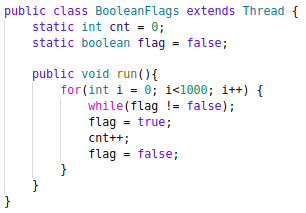
\includegraphics[scale=0.45]{BooleanFlags.png}
    \end{figure}
    \noindent When running the program with two threads the counter turns out to be unexpectedly low.\\[3mm]
    Looking at the implementation, we see that the critical section is in between the \texttt{flag = true} and \texttt{flag = false} statements. >The problem here is that there is a possible execution of the two threads, namely when both read \texttt{flag == false} before either of them could set \texttt{flag = true}, where both threads enter the critical section. Therefore, the second requirement of mutual exclusiveness is violated and this implementation is incorrect. 
\end{example}

\noindent As a final note, it's important to mention \textbf{livelocks}. Livelock occurs when all or at least some threads are changing state, but none of them actually enter the critical section. One might think of this visually as two people in a narrow hallway continuously trying to get past each other by stepping aside, but always stepping in the same direction. Note that a livelock doesn't mean that there is no possible execution which results in a thread entering the critical section, but simply that there is the possibility of the threads returning to the same state without any thread entering the critical section. This also implies that the algorithm isn't deadlock-free by definition.\\

%==============================================================================================================================

\subsubsection{State Diagrams}
An execution state diagram visually represents the different states and state transitions between them a particular program might go through. A program state is determined by the instructions the threads are executing and the states of global variables and concurrent objects. A state transition is then simply represented by arrows between such boxes.
\begin{example}
    We continue the previous example and construct the state diagram corresponding to the given code snippet, where we restrict ourselves to two threads for simplicity. We represent a state by a tuple (p$i$, q$j$, $b$) for $i,j \in \{1,2,3\}$ and $b \in \{0,1\}$.\\
    p$i$ resp. q$j$ represents the instruction the corresponding thread $P$ or $Q$ is about to execute. The represented instructions are:
    \begin{itemize}
        \item $i = 1$: \texttt{while(flag != false);}
        \item $i = 2$: \texttt{flag = true;}
        \item $i = 3$: \texttt{cnt++;}
    \end{itemize}
    $b$ represents the value of \texttt{flag}.
    \begin{figure}[H]
        \centering
        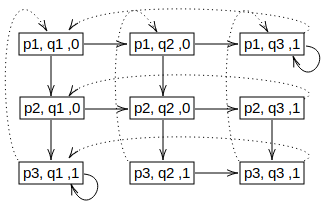
\includegraphics[scale=0.6]{FiniteStateDiagram.png}
    \end{figure}
    \noindent We see that there is indeed a path of state transitions leading to a state in which both threads are in the critical section. Therefore, the code doesn't provide mutual exclusion.
\end{example}
As you might have noticed, we omitted/summarized non-critical states for the sake of brevity.\\[3mm]
Using this state transition diagram, we can now easily recognize whether the critical section is implemented correctly.
\begin{itemize}
    \item \textbf{Deadlocks} can be recognized by states which have no outgoing state transitions.
    \item \textbf{Livelocks} are any possible cycle of state transitions in which in none of the states a thread is in the critical sections.
    \item The critical section is \textbf{mutually exclusive} if there is no state in which more than one thread is in the critical section.
\end{itemize}
\newpage

%==============================================================================================================================
%==============================================================================================================================

% Very short - essentially just the different implementations and an intuitive listing of advantages/disadvantages
\subsection{Mutex Implementation}
We will now look at different ways of actually implementing mutual exclusion. We will first look at different algorithms, always considering their advantages and disadvantages, then their efficiency on modern multiprocessors and how to improve further. To understand how these implementations were constructed or what the concrete proofs of the characteristics look like, one should consult the lecture slides or Chapter 2 of the book ''The Art of Multiprocessor Programming'' by Herlihy and Shavit.\\[3mm]
In the following, we assume all reads and writes are atomic. This assumption is necessary, as while we do add the \texttt{volatile} keyword to all array declarations, this only concerns the array references, not their entries. In practice, one would declare the arrays to be arrays of \texttt{AtomicInteger}s, i.e. as \texttt{AtomicIntegerArray}.

\subsubsection{Peterson Lock} \label{Peterson's Lock}
We assume only two threads attempt to acquire the lock, one with \texttt{ThreadID == 0} and the other with \texttt{ThreadID == 1}. The idea of the algorithm is as follows:
\begin{enumerate}
    \item Set our flag, thereby indicating that we're interested in entering the critical section.
    \item Indicate that the other thread is allowed to go first. The thread that arrives at this statement first will enter the critical section first.
    \item Wait until the other thread is either no longer interested in entering the critical section or until we're allowed to go first.
    \item Indicate that we're no longer interested.
\end{enumerate}
\begin{figure}[H]
    \centering
    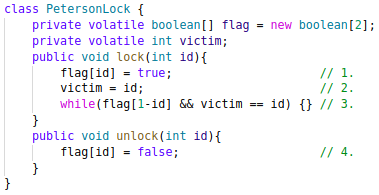
\includegraphics[scale=0.45]{PetersonLock.png}
\end{figure}
It's easy to see that the Peterson Lock satisfies the requirements for correct implementation of a critical section. In fact, it's even starvation-free. One can prove this using a short proof by contradiction.\\[3mm]
An obvious disadvantage of this implementation is that it only implements mutual exclusion for two threads. In most cases, we are interested in providing mutual exclusion for many more threads. The next section will adapt the Peterson Lock to do just that.

%==============================================================================================================================

\subsubsection{Filter Lock} \label{Filter Lock}
As mentioned in the previous section, the Filter Lock is a generalization of the Peterson Lock. In order to implement mutual exclusion for up to $n$ threads, we create $n-1$ ''levels'' that a thread must traverse (3) before entering the critical section. \\[3mm]
We generalize the notion of a two-element \texttt{flag} array with an $n$-element \texttt{level} array (1), where the value of \texttt{level[T]} indicates the highest level thread $T$ is trying to enter. Each level $k$ has an entry \texttt{victim[$k$]} (2), indicating that the thread specified in this entry wants to enter the level.\\[3mm]
Initially, a thread is at level 0. We say that $T$ is at level $k$ for $k>0$, when it completes the waiting loop (4) with $level[T]\geq k$. Note that this also means that a thread at level $k$ is also at level $k-1$ and so on. A thread can complete the waiting loop when another thread wants to enter its level or no more threads are in front of it.\\[3mm]
\begin{figure}[H]
    \centering
    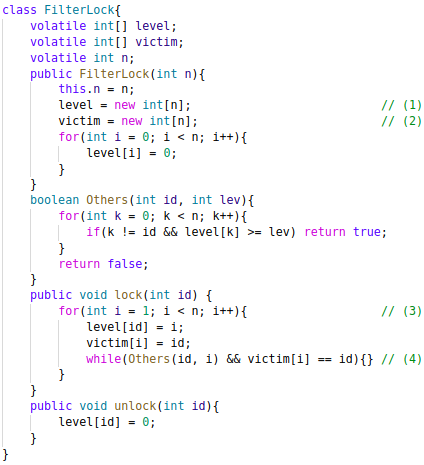
\includegraphics[scale=0.45]{FilterLock.png}
\end{figure}
\noindent We can prove by induction that for $k \in [0,n-1]$, there are at most $n-k$ threads at level $k$. Therefore, we can draw the key conclusion that at most 1 thread can be at level $n-1$, i.e. in the critical section. Again using induction, we can also show that the Filter Lock is starvation-free, which implies that it is also deadlock-free. In summary, the Filter Lock correctly implements mutual exclusion.\\[3mm]
However, one issue remains. We split the \texttt{lock()} method into two sections:
\begin{enumerate}
    \item A \textit{doorway} section, whose execution interval consists of a bounded number of steps.
    \item A \textit{waiting} section, whose execution interval may take an unbounded number of steps.
\end{enumerate}
We can now define a notion of fairness.
\begin{definition}
    A lock is \textit{first-come-first-served} if, whenever, thread $A$ finishes its doorway before thread $B$ starts its doorway, then $A$ cannot be overtaken by $B$.
\end{definition}
In the case of the \texttt{FilterLock} we can define the first two instructions of the for-loop to be the doorway and the waiting loop to be the waiting section. Finding an execution which doesn't adhere to the above definition is left as an exercise.\\[3mm]
In summary, the \texttt{FilterLock} does implement starvation-free mutual exclusion, but isn't fair according to the \textit{first-come-first-served} principle.

%==============================================================================================================================

\subsubsection{Bakery Lock}
The Bakery Lock is inspired by the number-dispensing machines often found in bakeries (or in the case of Switzerland: Post offices).\\[3mm]
The implementation is relatively straightforward: We have a \texttt{flag} array, indicating whether the thread want to enter the critical section or not, and a \texttt{label} array, where $label[i]$ contains the label assigned to the thread with $ThreadID == i$. In the \textit{doorway} section, we take a label, which is the current highest label incremented by one, and set our entry in the \texttt{flag} array. Note that several threads can receive the same label at this point. We then remain in the \textit{waiting} section until we have the lowest label (or in the case of identical labels: the lowest id) among all threads wanting to enter the critical section. 
\begin{figure}[H]
    \centering
    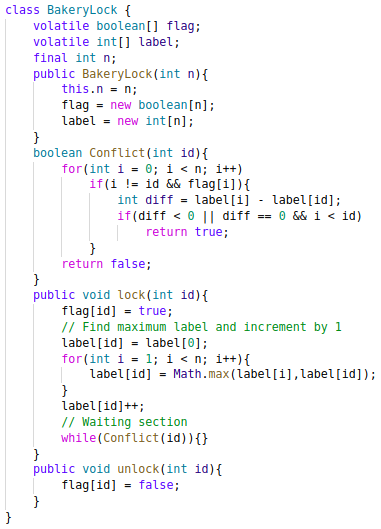
\includegraphics[scale=0.45]{BakeryLock.png}
\end{figure}
\noindent Proving that the \texttt{BakeryLock} is deadlock-free follows directly from the fact that the labels are strictly increasing and that the id assigned to each thread is unique. Therefore, there is always some thread with a unique (label, ThreadID) pair which is allowed to proceed into the critical section.\\[3mm]
It's very easy to see that the \texttt{BakeryLock} is also \textit{first-come-first-serve}, as once thread $A$ has finished the doorway section, any subsequent thread $B$ will always choose a higher label, thereby allowing $A$ to go first. Note that any algorithm that is both deadlock-free and \textit{first-come-first-serve} is also starvation-free.\\[3mm]
We can prove that the \texttt{BakeryLock} provides mutual exclusion using a proof by contradiction, where we make use of the uniqueness of the (label, ThreadID) pair.
 
%==============================================================================================================================

\subsubsection{Spin Lock}
When implementing mutual exclusion, there are two different choices on what to do when we cannot immediately acquire a lock. The first choice would be to continue trying to acquire the lock. This is called \textit{spinning} or \textit{busy waiting}. The \texttt{FilterLock} and \texttt{BakeryLock} are such spinlocks. As spinning takes up CPU cycles, this approach only makes sense on a multiprocessor system. The second choice would be to ask the operating system's scheduler to schedule another thread on your processor until the lock becomes available again. This is called \textit{blocking}. Because switching from thread to another is expensive, blocking only makes sense if you expect the lock delay to be long.\\[3mm]
Unfortunately, our lock implementations up until now won't work on most modern processors and compilers. This is because the compiler and the underlying hardware architecture do not guarantee memory operations to occur in-order. We tried to  somewhat alleviate this issue by introducing the \texttt{volatile} keyword, but this only guaranteed reads and writes to the array reference to be in-order, not to the entries of this array.\\[3mm]
We, therefore, arrive at a lock implementation using TAS and TTAS operations, which will be introduced in the sub-chapter ''Non-Blocking Algorithms'', for those unfamiliar with the concepts.
\begin{figure}[h]
    \centering
    \begin{subfigure}{.5\textwidth}
        \centering
        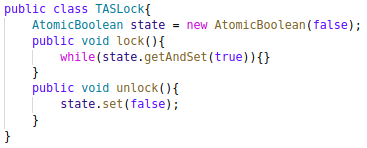
\includegraphics[scale=0.45]{TASLock.png}
    \end{subfigure}%
    \begin{subfigure}{.5\textwidth}
        \centering
        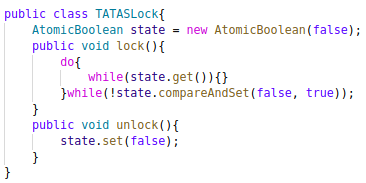
\includegraphics[scale=0.45]{TATASLock.png}
    \end{subfigure}
\end{figure}
When measuring performance, we see that both \texttt{TASLock} and \texttt{TATASLock}, while slightly better, both perform poorly. The reasons for this can be found in modern hardware architecture:
\begin{itemize}
    \item Calls to \texttt{getAndSet()} and \texttt{set()} force other processors to invalidate their cached copies of the \texttt{state} variable. This means that the next call to \texttt{get()} and \texttt{getAndSet()} will need to read from main memory. Continuing like this, it's easy to see that nearly every call will read from main memory.
    \item Nearly each call reading from main memory also means that the shared bus will be under heavy use. This means that all threads using the bus will be slowed down considerably.
\end{itemize}
The \texttt{TATASLock} performs slightly better, as the call to \texttt{get()} still tries to read from the local cached copy.\\[3mm]
One possibility to alleviate this problem would be to implement an exponential backoff. This means that every time we don't manage to acquire the lock, we wait for a random amount of time $m \in [0,t^x]$, where $x$ is the number of times we've failed to acquire the lock and $t$ is the initial wait time.

\newpage

%==============================================================================================================================
%==============================================================================================================================

\subsection{Synchronization}
As mentioned above, when we have a memory location which is neither thread-local nor immutable, we need to make sure we synchronize the resource properly across all threads. We, therefore, introduce the \texttt{synchronized} keyword. When a thread encounters the \texttt{synchronized} keyword, it will always first attempt to obtain the lock to the specified object. Until it obtains the lock, it will block.
\begin{example}
    We return to the example from section 3.2.1. Removing the incorrect synchronization primitive from the class and implementing mutual exclusion using the \texttt{synchronized} keyword gives us:
    \begin{figure}[H]
        \centering
        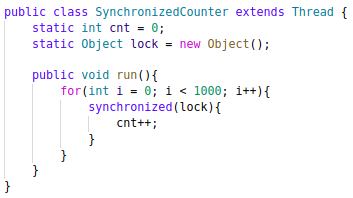
\includegraphics[scale=0.45]{SynchronizedCounter.png}
    \end{figure}
    \noindent Note that it's not possible to synchronize on a primitive value. One might be tempted to turn \texttt{cnt} into an \texttt{Integer}, but this would result in erroneous behavior. The reason for this is that primitive wrapper objects such as \texttt{Integer}s are immutable. Therefore, Java will create a new object every time we increment the \texttt{cnt} variable.
\end{example}
Every Java object, including classes itself, not just their instances, has an associated lock, meaning that we can use it to enforce mutual exclusion using \texttt{synchronized}. We can also include the \texttt{synchronized} in the method signature:
\begin{center}
    \texttt{public synchronized void someMethod()\{...\}}
\end{center}
This is equivalent to:
\begin{center}
    \texttt{public void someMethod() \{\ synchronized(this)\{...\}\ \}}
\end{center}
This means that before proceeding with the execution of the method body, we will first acquire the lock on the \texttt{this} object, which is either an instance of the class or the class itself if the method is declared \texttt{static}.\\[3mm]
Note that Java locks are reentrant.
\begin{definition}
    A lock is \textit{reentrant} if it can be acquired multiple times by the same thread.
\end{definition}
When creating a concurrent program with mutable, shared state, we think in terms of what operations need to be atomic. Locks do pretty much just that: Changes made inside of a \texttt{synchronized} block appear to other threads (provided they also acquire the lock before reading mutable, shared fields) to take place instantaneously. Nonetheless, locks aren't all rainbows and sunshine. When we have large critical sections which are all protected by locks, we reduce the parallelizable fraction in our program by a lot. Thinking back to Amdahl's Law, we know that this drastically reduces the possible speedup of our program.

%==============================================================================================================================

\subsubsection{Conditions}
% wait, notify, notifAll + Lock Condition interface --> Several waiting queues
Quite often, one might come across a case where a thread is only allowed to proceed once a certain condition has been met. One might be tempted to put the condition in a while-loop and let the thread spin until the condition is fulfilled. This solution, however, would be grossly inefficient, as this spinning thread would still be taking up a lot of CPU cycles, thereby slowing down all other threads.\\[3mm]
Lucky for us, Java locks provide methods created for this exact purpose. All of the following methods can only be called inside of a \texttt{synchronized} block, i.e. when the thread holds the lock.
\begin{itemize}
    \item \texttt{wait()}: Thread is moved into an inactive state and is inserted into the waiting queue. The thread releases the lock on which \texttt{wait()} was called.
    \item \texttt{notify()}: Some thread is removed from the waiting queue and moved into an active state. The thread that was just woken up will then proceed to attempt to re-acquire the lock normally. Note that we do not have any control over what thread is woken up.
    \item \texttt{notifyAll()}: All threads are removed from the waiting queue and moved into an active state. All these threads will then proceed to attempt to re-acquire the lock.
\end{itemize}
A very important thing to remember here is that the operating system might randomly wake up a waiting thread (spurious wakeups) or another thread might interrupt the waiting thread. Both of these cases would lead to the thread being woken up, possibly with an \texttt{InterruptedException}. To prevent the thread from continuing execution normally despite the condition not being fulfilled, we need to put it in a while-loop, as opposed to a simple if-statement.\\[3mm]
The \texttt{java.util.concurrent.locks} library also provides similar methods. In order to use them, we first need to create a \texttt{Condition} object, on which we can then call \texttt{await()}, \texttt{signal()} and \texttt{signalAll()}. The definitions for these three methods are identical to the ones listed above provided by the \texttt{synchronized} primitive, but for the separation of waiting queues. Instead of associating a waiting queue with a lock, we associate it with the \texttt{Condition} object. This means that we can have several waiting queues for a single lock. The advantage of this will become clear momentarily.\\[3mm]
There are two very important rules to using \texttt{wait()}/\texttt{notify()}:
\begin{enumerate}
    \item \textbf{Always} enclose a \texttt{wait()} statement in a \texttt{while} loop. The reason for this is that the operating system may randomly wake up a thread, without us having ever called \texttt{notify()}. These events are called \textit{spurious wakeups}. In addition, \texttt{notifyAll()} wakes up \textit{all} threads, meaning also those for which the entry condition might not have been fulfilled, yet.
    \item \textbf{Only} call \texttt{wait()} or \texttt{notify()} when holding the lock to the corresponding object. Java will throw an exception otherwise.
\end{enumerate}
The two rules listed above also hold for the \texttt{Condition} interface.
\begin{example}
    Let's say we work for some nameless company housed in a concrete monolith. The company has received complaints from the basement-housed employees that the nearest women's bathroom is two floors up. We're tasked with converting the basement's men's bathroom to a unisex bathroom, with the following constraints:
    \begin{itemize}
        \item There cannot be men and women in the bathroom at the same time.
        \item There should never be more than three employees squandering company time in the bathroom.
    \end{itemize}
    All of this, of course, without causing a deadlock.\\
    We came up with a system which allows whoever is standing outside of the bathroom to tell how many people and of which gender are inside. Therefore, the protocol for entering and exiting the bathroom will look as specified in the code.\\[3mm]
    This problem allows for a very nice visual interpretation of the difference between using \texttt{wait()}/\texttt{notify()} and using \texttt{Condition}s. The implementation using \texttt{wait()}/\texttt{notify()} creates a single queue in front of the bathroom entrance. Whenever someone leaves the bathroom, everybody in the queue will try to enter the bathroom. If they see that they can't, i.e. one of the requirements listed above doesn't hold, they'll get back in the queue. Otherwise, they'll enter the bathroom.\\[3mm]
    By contrast, using the \texttt{Condition} interface allows us to split this queue into two queues, one for male employees and the other for female employees. Whenever someone leaves the bathroom, they'll tell one of the queues that they're allowed to try and enter the bathroom. In order to have some fairness, when an employee is the last person to leave the bathroom, they'll always \texttt{signal} the queue of the opposite gender.
    \begin{figure}[H]
        \centering
        \begin{subfigure}{.5\textwidth}
            \centering
            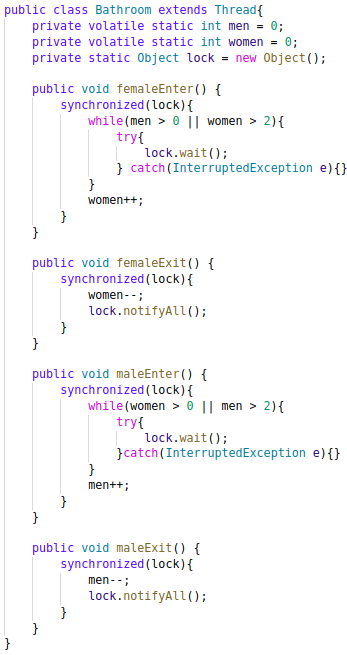
\includegraphics[scale=0.45]{BathroomwWait.png}
        \end{subfigure}%
        \begin{subfigure}{.5\textwidth}
            \centering
            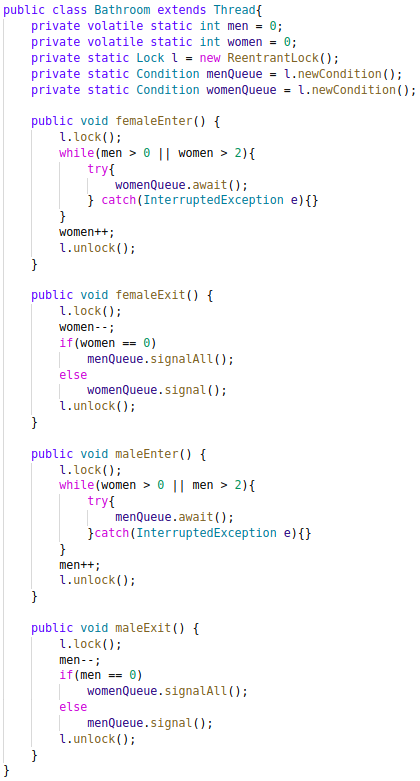
\includegraphics[scale=0.45]{BathroomwConditions.png}
        \end{subfigure}
    \end{figure}
\end{example}
It's important to note that even when the creation of several waiting queues could, in theory, be a lot more efficient, the \texttt{synchronized} primitive is implemented so much more efficiently in Java, that using the \texttt{Condition} interface is usually not worth the effort.

%==============================================================================================================================

\subsubsection{Semaphores}
% Idea and how to implement
Up until now, locks have always ensured that only a single thread enters the critical section. Yet in some cases, this might not be what we want. If, for example, we have a server that can support up to 100 requests at a time, we want to be able to allow up to 100 threads into the critical section. This is where semaphores come into play.\\[3mm]
A semaphore is a generalization of mutual exclusion locks. Each semaphore S has a capacity of $N$ and provides the following operations:
\begin{itemize}
    \item \texttt{acquire(S)}: Blocks until $N > 0$, then decrements $N$.
    \item \texttt{release(S)}: Increments $N$.
\end{itemize}
Note that both operations above should be considered to be atomic, to avoid data race or bad interleavings. The simplest approach to implementing semaphores is, therefore, to associate a lock with the two methods. Implementing a semaphore is left as an exercise.

%==============================================================================================================================

\subsubsection{Barriers}
% Idea and how to implement
We now want to go one step further. We wish to create a barrier which blocks all threads up until a certain threshold of $N$ threads. Once the threshold has been reached all threads waiting in the barrier are allowed to continue execution. We distinguish between non-reusable and reusable barriers. Note that in reusable barriers, we, next to correctly resetting the barrier to its initial state, have to deal with the issue that threads might attempt to re-enter the barrier while the other ones are still ''draining'' out.\\[3mm]

\newpage

\begin{wrapfigure}{r}{0.35\textwidth} %this figure will be at the right
    \centering
    \vspace{-10pt}
    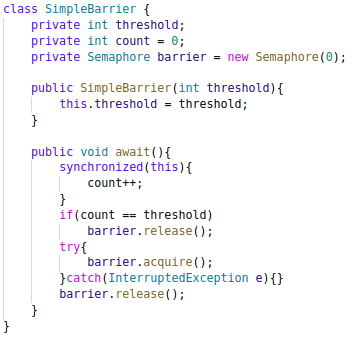
\includegraphics[scale=0.45]{SimpleBarrier.png}
\end{wrapfigure}
\vspace{0pt}
\noindent The non-reusable barrier has a relatively simple implementation, which can be seen in Fig. 1. Each arriving thread increments the counter (taking the lock to avoid race conditions) and attempts to acquire the \texttt{barrier} semaphore, thereby going into a blocked state. Once all threads have arrived, i.e. \texttt{count == threshold}, the \texttt{barrier} semaphore is set to 1, allowing one thread to pass. Whenever a thread passes the barrier it immediately releases it again so that the next thread may proceed with its execution. This method of acquiring and releasing the \texttt{barrier} semaphore is called a \textit{turnstile}.\\[3mm]


\noindent The reusable barrier is implemented in such a way that it can be reused once all waiting threads are released. To simplify our implementation, we assume no additional threads call the \texttt{await()} method before all waiting threads have been released.\\
The reusable barrier consists of two parts. First, the threads increment the counter, attempt to acquire the \texttt{barrier1} semaphore and go into a blocking state. Once the threshold is reached the \texttt{barrier1} semaphore is incremented so that the threads are allowed to pass the turnstile and enter the second part of the barrier. Additionally, the \texttt{barrier2} semaphore is decremented, thereby making the second part of the barrier behave identically to the first part, only now decreasing the counter. In the second part of the barrier, threads will be allowed to pass the turnstile once the counter's value is 0.\\
Note that once all threads have exited the barrier, all values have been restored to their original state, thereby allowing the barrier to be reused again.\\[3mm]
At this point, the reader is encouraged to think about why the different parts are necessary and what could go wrong if we changed anything about them. For example, what happens when a thread that has just left the barrier tries to re-enter? Will it overtake the other threads? If not, what prevents it from doing so?
\begin{figure}[H]
    \centering
    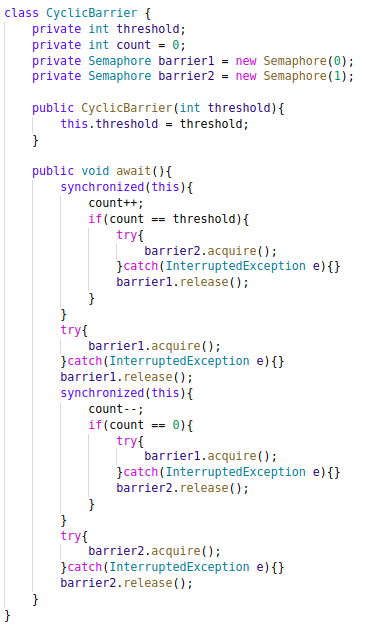
\includegraphics[scale=0.45]{CyclicBarrier.png}
\end{figure}
\newpage

%==============================================================================================================================
%==============================================================================================================================


\subsection{Lock Granularity}
% What's bad about locks, how to move to non-blocking algorithms
We've seen that the size of our critical section greatly influences the possible speedup we can achieve through parallelization. When programming with locks, it's common practice to start off essentially wrapping everything that remotely resembles a critical section in one huge lock. This is called \textit{coarse-grained locking}. In this sub-section, we introduce different locking strategies which, with some customization, can be applied to many different concurrent data structures. We introduce these strategies at the hand of sorted linked lists. 
\begin{example}
    A sorted linked list implements the following methods
    \begin{itemize}
        \item \texttt{add(x)}: adds \texttt{x} to the list in the position corresponding to the lexicographic ordering of x, returning \texttt{false} if \texttt{x} is already contained in the list.
        \item \texttt{remove(x)}: removes \texttt{x} from the list, returning \texttt{false} if the list doesn't contain \texttt{x}.
        \item \texttt{contains(x)}: returns \texttt{true} if the list contains \texttt{x}.
    \end{itemize}
\end{example}

\subsubsection{Coarse-Grained Locking}
With \textit{coarse-grained locking}, we take the sequential implementation of the data structure and synchronize all of its methods.
\begin{example}
    We only show the \texttt{remove} method for brevity:
    \begin{figure}[H]
        \centering
        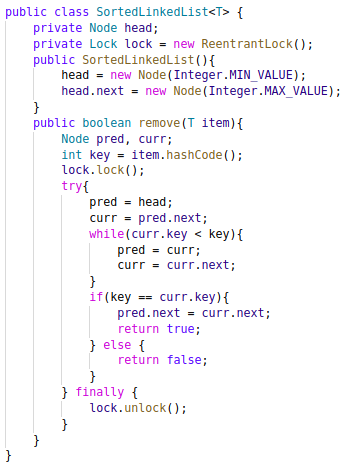
\includegraphics[scale=0.45]{CoarseGrained.png}
    \end{figure}
\end{example}
The disadvantage here is the considerable size of the critical section. As all the methods share a single lock and start by acquiring and end by releasing it, this implementation allows for barely any concurrency whatsoever. However, this strategy does have one advantage: its simplicity. Implementing it doesn't require any effort on the side of the programmer.
\newpage

%==============================================================================================================================

\subsubsection{Fine-Grained Locking} \label{fine-grained locking}
As a first step of improving \textit{coarse-grained locking}, we can lock individual elements instead of the entire data structure. As a thread traverses the data structure, it locks each node when it first visits it and releases it once it has acquired the lock for the next node. This method of locking is called \textit{hand-over-hand} locking. This method allows threads to traverse the data structure in a pipelined fashion.\\[3mm]
To avoid deadlocks, all threads must acquire the locks in some predefined order, e.g. in the case of the sorted linked list, all threads start at the head and don't try to ''skip'' nodes. 
\begin{example}
    In order to avoid deadlocks, it's important that all threads acquire the locks in some predefined order. In the case of sorted linked lists, this requirement is easily met by always starting at the \texttt{head} sentinel and only proceeding in a hand-over-hand fashion.
    \begin{figure}[H]
        \centering
        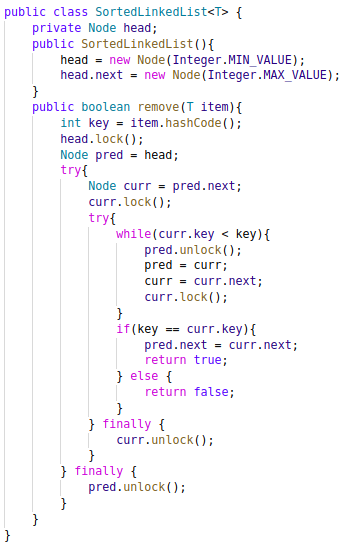
\includegraphics[scale=0.45]{FineGrained.png}
    \end{figure}
\end{example}
We've now implemented an actual concurrent data structure, in the sense that several threads can operate on it simultaneously. But unfortunately, this strategy is still far from perfect. As threads iterate over this data structure in a pipelined fashion, the slowest thread sets the tempo for all threads that immediately follow it, meaning that a potentially ''fast'' thread might experience a considerable slowdown. Also, for large data structures, there is still a potentially long chain of lock acquisitions and releases.

%==============================================================================================================================

\subsubsection{Optimistic Locking} \label{optimistic locking}
With \textit{optimistic locking}, we take somewhat of a risk. We iterate the data structure without taking any locks. Once we've found the required elements we lock them and check if everything is still correct. If we find that in-between finding the elements and taking the locks the state of the data structure changed to one where we can't execute our operation reliably anymore, we start over. As such conflicts are rare, we consider this approach to be optimistic.\\[3mm]
Implementing such a verification method is non-trivial and requires careful thought. What state do we, as an operating thread, \textit{expect} and how can we check that this expected state actually holds?
\newpage
\begin{example}
    In the case of the sorted linked list, we verify the following two conditions:
    \begin{itemize}
        \item The \texttt{curr} node, i.e. the node we're operating on, is still reachable.
        \item \texttt{pred} still points to \texttt{curr}, i.e. the two nodes we're about to operate on are actually the ones we \textit{should} operate on.
    \end{itemize}
    The reader is encouraged to check for themselves whether these two conditions are sufficient to guarantee a correct execution, e.g. by removing or weakening one condition and finding a case that would result in an incorrect execution.
    \begin{figure}[H]
        \centering
        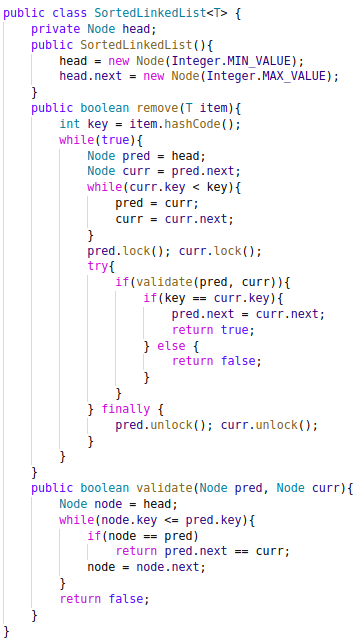
\includegraphics[scale=0.45]{OptimisticLocking.png}
    \end{figure}
\end{example}
We've now been able to alleviate most issues. Nonetheless, a few remain. First, by always calling \texttt{validate}, we're essentially iterating the list twice. If we then have a high amount of thread contention, i.e. a lot of threads operating on the same area of the data structure, these \texttt{validate} will often return \texttt{false}, thereby forcing most threads to re-iterate the entire list. Finally, we would like an operation as simple as the \texttt{contains} method to not have to acquire any locks whatsoever, as this does seem like a slight overkill.

%==============================================================================================================================

\subsubsection{Lazy Locking}
\textit{Lazy synchronization} builds on top of optimistic synchronization by adding a boolean \texttt{marked} field to each node, which - when \texttt{false} - holds the invariant that
\begin{itemize}
    \item the node is in the set and
    \item the node is reachable.
\end{itemize}
The \texttt{remove} method now first \textit{lazily} removes a node by setting its \texttt{marked} bit, then \textit{physically} removes it, e.g. by redirecting the pointer from the previous node. We adjust the \texttt{validate} method so that it only checks whether the \texttt{marked} bit is set and whether the local state is still as expected. Therefore, the remainder of the \texttt{add} and \texttt{remove} methods can be left the same. Finally, we change the \texttt{contains} method such that it simply iterates the data structure without taking any locks and, if it finds the specified node, checks whether it's marked or not.

\newpage

\begin{example}
    The concrete implementation of the sorted linked list according to the lazy locking strategy now looks as follows.
    \begin{figure}[H]
        \centering
        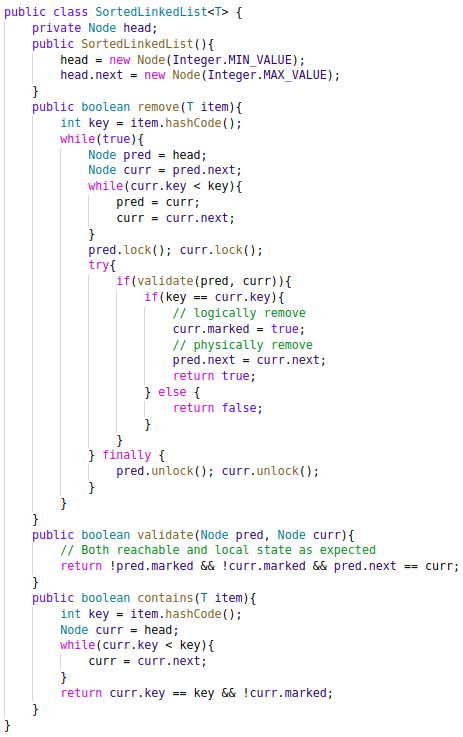
\includegraphics[scale=0.45]{LazyLocking.png}
    \end{figure}
\end{example}

\newpage

%==============================================================================================================================
%==============================================================================================================================

\subsection{Non-Blocking Algorithms}
While locks allow us to relatively easily make an operation atomic, there are still several important disadvantages to locking:
\begin{enumerate}
    \item Locks are \textbf{pessimistic} by design i.e. they assume the worst and enforce mutual exclusion
    \item Severe \textbf{performance issues}: Even when uncontested, a lock acquisition must read and write from main memory. When the lock is contested, this degradation becomes much worse.
    \item Locking is \textbf{hard}. A delayed thread might slow down all subsequent threads, deadlocks might occur, interrupt handlers become much harder to implement correctly, etc.
\end{enumerate}
We, therefore, strive to create operations and data structures that don't use any locks whatsoever. To see how we can implement these we'll first have a very quick look at the most important different atomic primitives, which are also provided by the Java \texttt{java.util.concurrent} library. Then we'll direct our attention to implementing an actual lock-free concurrent data structure and the problems that might occur when implementing one.

\subsubsection{Atomic Operations}
% TAS, CAS, AtomicmarkableReference, DCAS
All of the following methods are provided by the \texttt{java.util.concurrent.atomic} package. Note that some of them are not available in other programming languages.\\[3mm]
The \texttt{testAndSet()} operation takes a byte or word which represents a boolean value, reads the stored boolean value and stores the value for \texttt{true}. It then returns the previously read value. We've already seen how we can implement a simple spin lock using this atomic operation.\\[3mm]
The \texttt{compareAndSet()} method takes two arguments: an \textit{expected} value and an \textit{update} value. If the current stored value is equal to the expected value, it updates it to the specified update value, otherwise the value is left unchanged. Finally, it returns a boolean value indicating whether the value was replaced or not.\\
\begin{figure}[H]
    \centering
    \begin{subfigure}{.5\textwidth}
        \centering
        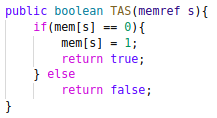
\includegraphics[scale=0.45]{TAS.png}
    \end{subfigure}%
    \begin{subfigure}{.5\textwidth}
        \centering
        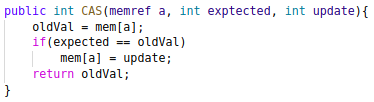
\includegraphics[scale=0.45]{CAS.png}
    \end{subfigure}
\end{figure}
\noindent An \texttt{AtomicMarkableReference<T>} is an object that encapsulates both a reference to an object of type \texttt{T} and a boolean \texttt{mark} bit. Both of these fields can be updated atomically, either alone or both at once.\\
This leads us to a new version of the \texttt{compareAndSwap()} operation, namely the so-called double compare-and-swap, which takes four values: two \textit{expected} values and two \textit{update} values. It atomically checks whether both the reference and the mark bit are as expected, replaces them by the update values if so and returns a boolean value indicating whether the values were replaced or not.\\
It also provides the \texttt{attemptMark(T expectedReference, boolean newMark)} method, which checks whether the reference is as expected and, if it is, replaces the mark bit. \\
Finally, it's important to mention that the \texttt{get(boolean[] marked)} has a somewhat unusual interface, as it returns the object's reference value and stores the mark value in the boolean array which was passed as an argument.

%==============================================================================================================================

\subsubsection{ABA-Problem}
% Show lock-free stack implementation
Several different lock-free data structures were introduced during the lectures. For the sake of brevity, we'll focus on a lock-free stack implementation here.\\[3mm]
\newpage
Using the atomic operations introduced above, we can relatively easily implement a lock-free stack:
\begin{figure}[H]
    \centering
    \begin{subfigure}{.5\textwidth}
        \centering
        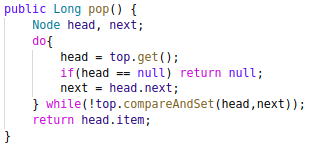
\includegraphics[scale=0.45]{StackPop.png}
    \end{subfigure}%
    \begin{subfigure}{.5\textwidth}
        \centering
        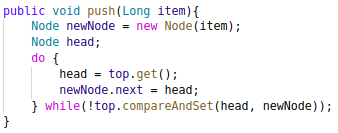
\includegraphics[scale=0.45]{StackPush.png}
    \end{subfigure}
\end{figure}
\noindent We see that we create a new node for every single \texttt{push} operation. As an optimization, we implement a node pool which allows for reuse of the node objects:
\begin{figure}[H]
    \centering
    \begin{subfigure}{.5\textwidth}
        \centering
        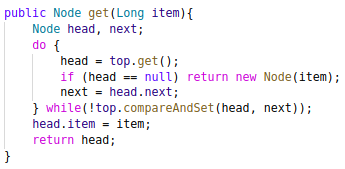
\includegraphics[scale=0.45]{NodePoolGet.png}
    \end{subfigure}%
    \begin{subfigure}{.5\textwidth}
        \centering
        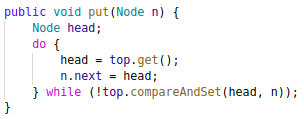
\includegraphics[scale=0.45]{NodePoolPut.png}
    \end{subfigure}
\end{figure}
\noindent When we adjust the stack implementation to use such a \texttt{NodePool}, we do indeed see a massive improvement in execution time. However, we see that the program exhibits erroneous behavior for some runs. This leads to a very common problem in lock-free concurrent programming, the \textbf{ABA Problem}.
\begin{definition}
    The ABA problem occurs when one activity fails to recognize that a single memory location was modified temporarily by another activity and therefore erroneously assumes that the overall state has not been changed.
\end{definition}
In the case of the lock-free stack with node reuse, this means the following scenario would exhibit an ABA-problem: We try to \texttt{pop} and observe that \texttt{head == a} and \texttt{head.next == b}. We then try to compare-and-set \texttt{head} to \texttt{b}. Suppose however, that another thread removes both \texttt{a} and \texttt{b}, pushes some other node \texttt{c} and then pushes \texttt{a}. We would then observe \texttt{head == a} as expected and set \texttt{head == b}, a node which is possibly not even in the stack at the time.\\[3mm]
There are several possible alternatives to alleviate the ABA problem:
\begin{itemize}
    \item \textbf{DCAS}: We can check whether both \texttt{head} and \texttt{head.next} are as expected, but doesn't exist on most platforms.
    \item \textbf{Garbage Collection}: Would eliminate the need for a \texttt{NodePool}, but is very slow and doesn't always exist either.
    \item \textbf{Pointer Tagging}: By incrementing the address bits made available by alignment, we can decrease the odds of the ABA problem occuring by a lot. Nonetheless, this doesn't actually alleviate the problem, only delay it.
    \item \textbf{Hazard Pointers}: We can associate an \texttt{AtomicReferenceArray<Node>} with the data structure where we temporarily store references which we've read and wish to write to in the future. Whenever we return a Node to the \texttt{NodePool}, we check whether its reference is stored in the \texttt{hazarduous} array. While this solution does work, the final product of a \texttt{NodePool} doesn't really improve performance when compared to regular memory allocation with a garbage collector. 
\end{itemize}

\newpage

%==============================================================================================================================
%==============================================================================================================================

\subsection{Linearizability and Sequential Consistency}
We've now looked at many different ways of implementing both blocking and non-blocking concurrent data structures and ensuring correctness. Interestingly enough, we did all this without ever properly defining what a correct parallel execution is. That is the aim of this section, defining different notions of correctness, some more strict than others, so that we may argue and prove things about our implementations.

\subsubsection{Histories}
We won't argue about implementations as a whole just yet. First, we'll consider one specific execution, called a \textit{history}, and argue whether this specific history is correct.\\[3mm]
A \textbf{method call} consists of a method \textit{invocation} and \textit{response}. An invocation that has no matching response is called \textit{pending}. A \textbf{history} is a finite sequence of method invocations and responses. A \textbf{subhistory} is a subsequence of the events. \textit{complete(\textbf{H})} is the subsequence of a history \textbf{H} consisting of all matching invocation and response events in \textbf{H}. A history is \textit{sequential} if every invocation is immediately followed by a matching response, i.e. when no method calls overlap.\\[3mm]
\begin{example}
    We're given the following history:
    \begin{figure}[H]
        \centering
        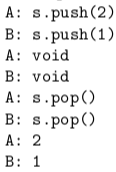
\includegraphics[scale=0.5]{History.png}
    \end{figure}
    \noindent We can see that the first two method calls and the last two method calls overlap.\\
    An easy visualization of histories is through the use of time lines. In this case, it could look like this:\\[3mm]
    \texttt{
        A s.push(1):\hspace{6pt}*--------------*\\
        B s.push(2):\hspace{30pt}*-------------*\\
        B s.pop()->1:\hspace{170pt}*----------------------*\\
        A s.pop()->2:\hspace{200pt}*-------------------*\\
    }
    There are many possibilities of representing a given history with a timeline, as we have no way of telling how long a specific method call might take compared to others or how much time passes in between method calls.
\end{example}
We say that method call $m_0$ precedes a method call $m_1$ if $m_0$ finished before $m_1$ started, i.e. $m_0$'s response event occurs before $m_1$'s invocation event. We denote this by $m_0 \rightarrow_H m_1$.

%==============================================================================================================================

\subsubsection{Sequential Consistency} \label{sequentially consistent}
\begin{definition}
    A program must fulfill two requirements to be deemed \textbf{sequentially consistent}:
    \begin{itemize}
        \item Method calls should appear to happen in a \textbf{one-at-a-time, sequential order}. This means that given a history \textbf{H}, every \textit{thread subhistory} is a sequential history, i.e. every method call returns before the next one starts.
        \item Method calls should appear to take effect in \textbf{program order}. This means that we can order all method calls such that they
            \begin{enumerate}
                \item are consistent with respect to the program order, i.e. they adhere to the ordering imposed by the thread subhistories
                \item meet the object's sequential specification
            \end{enumerate} 
    \end{itemize} 
\end{definition}
Note that it's possible for a history to have several possible sequential orderings such that the above holds.
\begin{example}
    We continue our example from the previous section and check whether the history is sequentially consistent.\\[3mm]
    The first requirement states that method calls should appear to happen in a one-at-a-time, sequential order, i.e. that every thread subhistory is a sequential history. Indeed, we see that this requirement holds for both thread subhistories \texttt{H$\mid$A} and \texttt{H$\mid$B}, i.e. each method call finishes before the next one starts.\\[3mm]
    The second requirement asks us to find a method call ordering such that they are consistent w.r.t. program order and they meet the object's sequential specification. One such ordering is given by
    \begin{center}
        \texttt{s.push(1) $\rightarrow$ s.push(2) $\rightarrow$ s.pop()->2 $\rightarrow$ s.pop()->1}
    \end{center}
    Note that this is not the only possible ordering. Another possibility would've been
    \begin{center}
        \texttt{s.push(2) $\rightarrow$ s.push(1) $\rightarrow$ s.pop()->1 $\rightarrow$ s.pop()->2}
    \end{center}
    Recognizing that progam order, i.e. thread subhistories, is repsected by both of these orderings, is left up to the reader as an exercise.
\end{example}

%==============================================================================================================================

\subsubsection{Linearizability} \label{linearizable}
The idea behind linearizability is that the concurrent history is equivalent to some sequential history. The rule is that if one method call precedes another, then the earlier call must have taken effect before the later call. By contrast, if two method calls overlap,  then their order is ambiguous, and we are free to order them in any convenient way.
\begin{definition}
    A history \textbf{H} is linearizable if it has an extension \textbf{H'} such that \textbf{H'} is complete and there is a legal sequential history \textbf{S} such that
    \begin{enumerate}
        \item complete(H') is equivalent to \textbf{S}, and
        \item if $m_0 \rightarrow_H m_1$, then $m_0 \rightarrow_S m_1$
    \end{enumerate}
\end{definition}
We can extend this notion by the following theorem:
\begin{theorem}
    \textbf{H} is linearizable if, and only if, for each object x, \textit{\textbf{H}$\mid$x}, i.e. the subhistory of \textbf{H} with only all method calls concerning object x, is linearizable.
\end{theorem}
Composability is important because we can design, implement and also prove things about concurrent systems in a modular fashion. Note that sequential consistency has no such property.
\newpage

%==============================================================================================================================
%==============================================================================================================================

\subsection{Consensus} \label{consensus protocol}
To bring this chapter to a close, we want to define a notion of how \textit{strong} a certain synchronization primitive, such as test-and-set, is. Using this we could, for example, show that there is an ordering on all synchronization primitives, such that no primitive at one level can be used for a wait-free or lock-free implementation of any primitives at higher levels. \\[3mm]
The idea is as follows: Each class in the hierarchy has an associated \textit{consensus number}, which is the maximum number of threads for which objects of the class can solve an elementary synchronization problem called \textit{consensus}. \\[3mm]
A \textit{consensus object} provides a single method \texttt{decide()}. Each thread calls the \texttt{decide()} method with its input v at most once. The object's \texttt{decide()} method will then return a value meeting the following conditions:
\begin{itemize}
    \item \textit{consistent}: all threads decide the same value
    \item \textit{valid}: the common decision value is some thread's input
\end{itemize}
In other words, a concurrent consensus object is linearizable to a sequential consensus object in which the thread whose value was chosen completes its call to  \texttt{decide()} first.\\[3mm]
We are interested in wait-free solutions to the consensus problem, that is, wait-free concurrent implementations of consensus objects. For historical reasons, any class that implements consensus in a wait-free manner is called a \textit{consensus protocol}. We say that a class \textbf{C} solves \textit{n-thread consensus} if there exists a consensus protocol using any number of objects of class \textbf{C} and any number of atomic registers. The \textit{consensus number} of a class \textbf{C} is the largest n for which that class solves n-thread consensus.\\[3mm]
A typical consensus protocol will look as follows:
\begin{figure}[H]
    \centering
    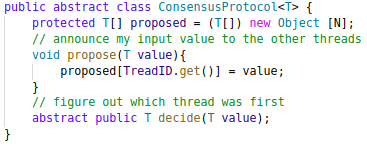
\includegraphics[scale=0.45]{ConsensusProtocol.png}
\end{figure}
Let's quickly have a look at what this would look like in an example:
\begin{example}
    We're given an atomic implementation of the test-and-set primitive as specified in the previous section. We wish to show that test-and-set solves 2-thread consensus. To that end, we construct the following consensus protocol:
    \begin{figure}[H]
        \centering
        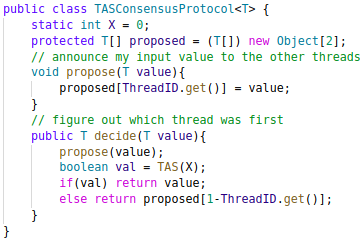
\includegraphics[scale=0.45]{TASConsensus.png}
    \end{figure}
    We see that the call to \texttt{TAS(X)} will only return \texttt{true} once, namely the first time it's called. Otherwise, it'll always return false. It's therefore easy to see that the returned result is both consistent and valid. As the protocol doesn't contain any loops or other dependencies, it's wait-free. Therefore, we've provided a correct 2-thread consensus protocol and shown that test-and-set implements 2-thread consensus.\\[3mm]
    Note that we can't extend this implementation to n-treads, as a ''loser'' thread has no way of telling which entry of the \texttt{proposed} array it should use. 
\end{example}
We've now defined what a consensus protocol is. Next, we would like to be able to prove things about concurrent objects using these consensus protocols, e.g. that a concurrent object solves \textit{at most} n-thread consensus for some n.\\[3mm]
A \textit{protocol state} consists of the states of the threads and the shared objects. When several threads call a consensus protocol, each thread makes \textit{moves} until it decides on a value. Here, a move is a method call to a shared object, i.e. a transition from one state to the next.\\
A wait-free protocol's set of possible states forms a tree of finite depth, where each node represents a possible protocol state and each edge represents a possible move by some thread.\\
In the case of \textit{binary consensus}, i.e. when the only possible decision values are 0 and 1, a protocol state is called \textit{bivalent} if the decision value is not yet fixed, i.e. several final states are reachable in which the decision value differ. In contrast, we call a protocol state \textit{univalent} if the outcome is fixed, i.e. all reachable final states decide on the same value. Finally, a \textit{critical state} is a bivalent state in which any move leads to a univalent state.
\begin{example}
    One of the most important proofs in concurrency theory using consensus protocols shows that, surprisingly, atomic registers have consensus number 1. Note that this doesn't mean that only one thread is allowed to try and access an atomic register at a time, it simply means that we can't solve n-thread consensus for n$>1$ using atomic registers. The proof roughly looks as follows:\\[3mm]
    Suppose there exists a binary consensus protocol for two threads \textbf{A} and \textbf{B}. As every consensus protocol is wait-free, it goes through a finite number of bivalent states. We can, therefore, run the protocol until we reach a critical state s. Assume \textbf{A}'s next move carries it to a 0-valent state and \textbf{B}'s next move to a 1-valent state. We will now consider an exhaustive list of the methods that they might be about to call to cause such a state transition.\\[3mm]
    \indent Suppose \textbf{A} is about to read a given register (we don't care about \textbf{B} here). Then there are two possible scenarios: either \textbf{B} moves first, carrying the protocol to a 1-valent state s', or \textbf{A} moves first, carrying the protocol to a 0-valent state s''. Let's say that in both cases \textbf{B} would then run solo, eventually deciding 0 or 1, respectively. But as the read \textbf{A} only changes its thread-local state, states s' and s'' should be indistinguishable to \textbf{B}, i.e. it should decide on the same value in both scenarios, a contradiction.\\
    \indent In the next case we consider, suppose that both threads are about to write to different registers, \textbf{A} to $r_0$ and \textbf{B} to $r_1$. Either \textbf{A} first writes to $r_0$ and \textbf{B} to $r_1$, carrying the protocol to 0-valent state, or \textbf{B} writes first, carrying the protocol to a 1-valent state. The problem is that, once again, the two resulting protocol states are indistinguishable from each other, which is a contradiction.\\
    \indent In the final case, suppose that both threads are about to write to the same register $r$. First, suppose that \textbf{A} writes first, carrying the protocol to a 0-valent state, and \textbf{B} then runs solo, eventually deciding 0. Second, suppose that \textbf{B} writes first and runs solo, therefore eventually deciding 1. The problem is that in both cases \textbf{B} overwrote whatever it is that \textbf{A} wrote into the register, i.e. \textbf{B} can't tell the difference between the two states. We've therefore reached another contradiction.\\[3mm]
    We've now shown that for all three possible types of consensus protocols one might construct using atomic registers, we reach a contradiction. It's therefore impossible to construct a 2-thread consensus protocol using atomic registers, i.e. atomic registers have consensus number 1.
\end{example}

In the proof above, one might be tempted to solve the problems leading contradictions using locks or by allowing one thread to go first, but then the protocol wouldn't be guaranteed to finish within in a bounded number of steps, i.e. it wouldn't be wait-free.
 
\newpage

%==============================================================================================================================
%==============================================================================================================================

\subsection{Exercises}
    \begin{ExerciseList}
        
        \Exercise[title={Mutual Exclusion},label=MEI].\quad A program is executed by two threads \textbf{A} and \textbf{B}. Each thread has three statements, labelled $a_i$ and $b_i$, respectively. Statements $a_3$ and $b_3$ correspond to the critical section. In the following state diagrams, each state is described by the current statement for each thread in the form $\{a_i,b_i\}$. Arrows show the possible state transitions.\\[3mm] 
        For each of the diagrams, decide whether the program implements mutual exclusion correctly. If not, argue what the problem(s) are. Distinguish between livelock and deadlock.
                
            \begin{figure}[H]
                \centering
                \begin{subfigure}{.5\textwidth}
                    \centering
                    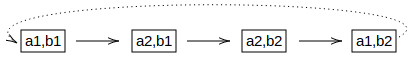
\includegraphics[scale=0.5]{STD1.png}
                    \captionsetup{labelformat=empty}
                    \caption{(i)}
                \end{subfigure}%
                \begin{subfigure}{.5\textwidth}
                    \centering
                    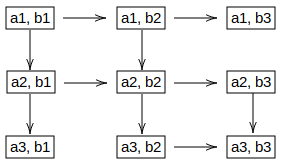
\includegraphics[scale=0.5]{STD2.png}
                    \captionsetup{labelformat=empty}
                    \caption{(ii)}
                \end{subfigure}
            \end{figure}
            
            \begin{figure}[H]
                \centering
                \begin{subfigure}{.5\textwidth}
                    \centering
                    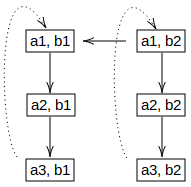
\includegraphics[scale=0.5]{STD3.png}
                    \captionsetup{labelformat=empty}
                    \caption{(iii)}
                \end{subfigure}%
                \begin{subfigure}{.5\textwidth}
                    \centering
                    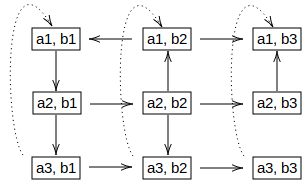
\includegraphics[scale=0.5]{STD4.png}
                    \captionsetup{labelformat=empty}
                    \caption{(iv)}
                \end{subfigure}
            \end{figure}
            
        \Answer[ref={MEI}].\quad \\
        \begin{enumerate}[label=(\roman*)]
            \item \quad While this implementation does provide mutual exclusion in the sense that no two processes are in the critical section at the same time, it's not correct either. We see that the processes continuously transition from one state to the next, without ever entering the critical section, i.e. this implementation contains a livelock.
            \item \quad This time around the implementation doesn't contain a dead- or livelock. However, we see that there is a path of state transitions, i.e. an execution, which results in both threads being in the critical section at the same time. Therefore, this implementation isn't correct.
            \item \quad We see that the threads never get stuck in a state and there is no path which doesn't result in one of the threads being in the critical section, i.e. the program contains neither a dead- nor a livelock. In addition, we see that there is no possible sequence of state transitions which results in both threads being in the critical section at the same time. Therefore, this implementation is correct. Note that thread \textbf{B} never enters the critical section. This doesn't mean the implementation is incorrect, only that it suffers from starvation.
            \item \quad We see that there is a cycle of state transition which doesn't result in one of the threads entering the critical section, i.e. the implementation suffers from livelock. In addition, there is a sequence of state transitions which results in both threads being in the critical section at the same time. In summary, this implementation suffers from livelock and doesn't provide mutual exclusion, i.e. it's incorrect.
        \end{enumerate}
        
        
        \Exercise[title={Progress Conditions},label=PC].\quad \\
            \Question Consider the following implementation of a concurrent stack's \texttt{push} method.
                \begin{figure}[H]
                    \centering
                    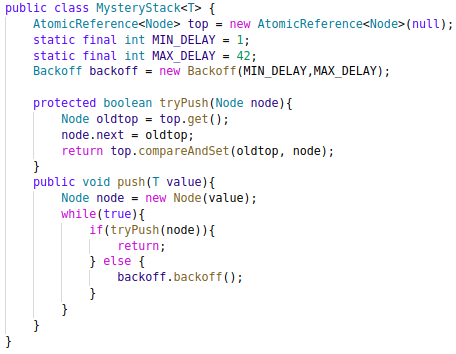
\includegraphics[scale=0.45]{MysteryStack.png}
                \end{figure}
                Name the \nameref{progress conditions} fulfilled by this implementation of the \texttt{push} method and describe your reasoning.
            \Question Prove that a wait-free program cannot use locks.
            \Question Suppose two cooks share a kitchen. In order to avoid both cooks using the same ingredient simultaneously (which would be really awkward), cooks need to know in advance what ingredients they need and then call the following program:
            \begin{figure}[H]
                \centering
                \begin{subfigure}{.5\textwidth}
                    \centering
                    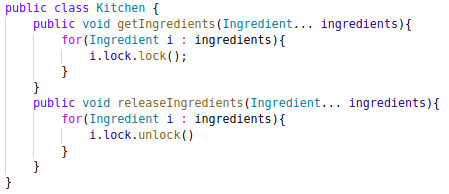
\includegraphics[scale=0.45]{Kitchen.png}
                \end{subfigure}%
                \begin{subfigure}{.5\textwidth}
                    \centering
                    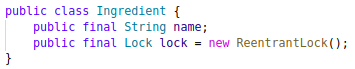
\includegraphics[scale=0.45]{Ingredient.png}
                \end{subfigure}
            \end{figure}
            What's the problem with this implementation? Describe a scenario that could cause the issue to occur and suggest a way to resolve it.
            
        \Answer[ref={PC}].\quad \\
            \Question We see that this implementation is identical to the lock-free stack implementation from section 3.5 with an added backoff mechanism. Nonetheless, an argumentation is required. \\[3mm]
            At no point during the execution of the \texttt{push} method does the thread transition into a blocked state. Therefore, this implementation must be lock-free. This also implies that it's deadlock-free. We do realize, however, that a thread isn't guaranteed to successfully push a node within a finite amount of time, e.g. when other threads keep popping/pushing nodes just before the thread calls \texttt{compareAndSet}. Therefore, this implementation isn't wait-free. In addition, this means that the method isn't starvation-free.
            \Question In a wait-free algorithm, any thread needs to be able to make progress independently of other threads. An algorithm is wait-free if every operation has a bound on the number of steps the algorithm will take before the operation completes. Thus, we cannot use locks to implement a wait-free algorithm (assuming locks are used to protect shared resources), as thread A might obtain the lock, then become really slow. During this period all other threads that want to obtain the lock are blocked and cannot make any progress.
            \Question This implementation suffers from deadlock. Suppose cook A wants to use ingredients $I_1$ and $I_2$ and cook B wants to use $I_2$ and $I_1$. Both proceed to call \texttt{getIngredients} simultaneously and obtain the first lock, i.e. cook A holds the lock for $I_1$ and cook B for $I_2$. Neither cook can now make progress as they are waiting for the other to release the lock.\\[3mm]
            One possible solution would be to impose an ordering on the ingredients in which their locks must be obtained. For example, we could enforce that locks must always be obtained in alphabetical order of the ingredients' names. Note that this assumes that no two ingredients have the same name, which is a sensible assumption to make when working in a kitchen.
        \pagebreak
            
        
        \Exercise[title={Peterson's},label=IP].\quad \\
            \Question Consider the following implementation of the \nameref{Peterson's Lock}.
                \begin{figure}[H]
                    \centering
                    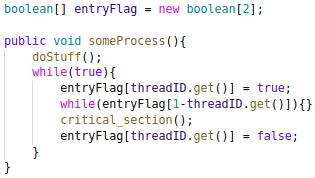
\includegraphics[scale=0.45]{badPeterson.png}
                \end{figure}
                Draw the state diagram with all the relevant states and decide, based on the diagram, whether this implementation is correct or not. If not, describe what the problem is.
            \Question Another way to generalize the two-thread Peterson lock is to arrange several 2-thread Peterson locks in a binary tree. Suppose $n$ is a power of two.\\[3mm]
                Each thread is assigned a leaf lock which it shares with one other thread. Each lock treats one thread as thread 0 and the other thread as thread 1.\\[3mm]
                In the tree-lock's \texttt{lock} method, the thread acquires every two-thread Peterson lock from that thread's leaf up to the root. The tree-lock's \texttt{unlock} method unlocks each of the 2-thread Peterson locks that thread has acquired, from the root back down to its leaf. At any time, a thread can be delayed for a finite duration (In other words, threads won't drop dead). For each property, either sketch a proof that it holds, or describe a (possibly infinite) execution where it's violated.
                \begin{enumerate}
                    \item Mutual exclusion
                    \item Freedom from deadlock
                    \item Freedom from starvation
                \end{enumerate}
        \Answer[ref={IP}].\quad \\
            \Question As can be read off the diagram below, this implementation suffers from livelock, e.g. when both threads reach the while-loop simultaneously. In this case, both threads would observe that the \texttt{entryFlag} field of the other thread is set and would therefore both decide to enter the while-loop. Therefore, this implementation is incorrect.
            \begin{figure}[H]
                \centering
                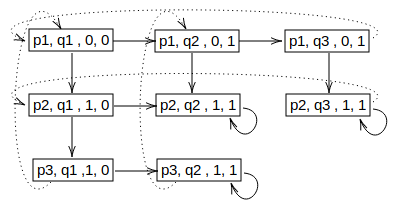
\includegraphics[scale=0.6]{STD5.png}
            \end{figure}
            \Question
                \begin{itemize}
                    \item \textbf{Mutual exclusion}: We see that only two threads share a single leaf node. As the Peterson lock provides mutual exclusion for two threads, the leaf node also provides mutual exclusion. If two subtrees of a single node both provide mutual exclusion, at most two threads can arrive at this node. As this node is also a Peterson lock, it provides mutual exclusion for two threads. By induction, we follow that this generalization of the Peterson's lock provides mutual exclusion.
                    \item \textbf{Freedom from deadlock}: Similarly, we show inductively that the generalization provides freedom from deadlock.
                    \item \textbf{Freedom from starvation}: This property is a bit trickier to prove (in fact, the solution from FS19's script incorrectly stated that the property didn't hold, until an attentive student showed otherwise). We consider trees of size $2^n$ and prove freedom from starvation by induction over $n\in \mathcal{N}$:\\[3mm]
                    \begin{itemize}
                        \item $n=1$: We have a tree of size $2^1$, i.e. two threads are attempting to acquire a single lock. The Peterson Lock is starvation free. Thus, starvation freedom holds for this case.
                        \item IH: Let $n>0$ be arbitrary. We assume the binary lock tree of size $2^n$ provides freedom from starvation.
                        \item Induction Step: We now show that the binary lock tree of size $2^(n+1)$ also provides freedom from starvation. Assuming $2^(n+1)$ threads, we can divide them into 2 groups of $2^n$ threads and manage them with trees of size $2^n$. \\
                        From IH, we are sure that each thread will acquire the root lock of its subtree at some point.
                        We now build the final tree by connecting roots of both subtrees to a final root lock $R$. Note that due to the setting of the \texttt{victim} field, the two subgroups will alternate in acquiring $R$.\\
                        Since any thread will acquire the root of its subtree, and since the final root lock is starvation free, we know that any thread will eventually acquire its subtree root, and finally $R$. This concludes the proof that the binary lock tree for $2^(n+1)$ threads is starvation free.
                    \end{itemize}
                \end{itemize}
        
        
        \Exercise[title={Fairness},label=Filter].\quad Recall the definition of \textit{first-come-first-served}: A lock is first-come-first-served if, whenever thread A finishes its doorway before thread B starts its doorway, A cannot be overtaken by B. \\[3mm]
        Describe an execution of the \nameref{Filter Lock} which doesn't adhere to the definition of first-come-first-served.
        \Answer[ref={Filter}].\quad Suppose $n = 3$, thread A is stuck at level 0, thread B at level 1 and thread C is at level 2, i.e. in the critical section. C finishes its critical section and releases the lock, thereby setting its level to 0. Now that there are no more threads at any higher levels, B enters the critical section. B finishes its critical section and also sets its level to 0. Let's say both B and C attempt to acquire the lock again, ending up with \texttt{victim[1] == C}. While A could, in theory, enter the next level, B might be faster and enter level 1 (and subsequently level 2, i.e. the critical section). Therefore, despite having completed the doorway section before B started its doorway sections, A was overtaken by B. Thus, the Filter Lock isn't fair.
        
        %TODO: Add exercise on barriers (build on "left as an exercise" mentioned in section)
        
        \Exercise[title={Lock Granularity},label=LG].\quad \\
            \Question Explain why the \nameref{fine-grained locking} algorithm isn't subject to deadlock.
            \Question Show a scenario in the \nameref{optimistic locking} algorithm where a thread is forever attempting to delete a node.
        \pagebreak
            
        \Answer[ref={LG}].\quad \\
            %Include example of swapping order in which pred and curr are locked in add method
            \Question For a deadlock to occur, the dependency graph must allow for a cyclic dependency. In the fine-grained locking algorithm, all threads obtain the locks in a set order. In the case of the sorted linked list, for example, all threads acquire locks in increasing order. Therefore, a cyclic dependency becomes impossible.\\[3mm]
            Suppose that the \texttt{add} method of the sorted linked list first acquired the lock for \texttt{curr}, then for \texttt{pred}. If another thread is executing the \texttt{remove} method, it might've already acquired the lock for \texttt{pred}, and be attempting to acquire the lock for \texttt{curr}. Both threads would be waiting for the other to release the lock. Thus, two threads acquiring locks in different orders can result in a deadlock.
            
            \Question Suppose thread A wishes to remove node c. It can happen that the \texttt{validate} method always returns \texttt{false}, thereby forcing A to always retry and never successfully remove c. A scenario in which the \texttt{validate} method always returns \texttt{false} would be when other threads are continuously adding and removing nodes in between c and its predecessor, i.e. the comparison \texttt{pred.next == curr} may evaluate to \texttt{false} everytime. As long as no other thread removes c, A will continue to try to remove c.

        
        \Exercise[title={Linearizability and Sequential Consistency},label=LSC].\quad \\
            \Question Draw a timeline for each of the following histories: \\
                \vspace{-10pt}
                \begin{multicols*}{3}
                    \texttt{
                        \noindent A: s.push(2)\\
                        B: s.top() \\
                        A: void \\
                        C: push(1) \\
                        C: void \\
                        B: 1 \\
                        C: s.push(2) \\
                        A: s.pop() \\
                        A: 1 \\
                        C: void \\
                        \columnbreak
                         \\
                        B: r.write(1) \\
                        A: r.read() \\
                        C: r.write(2) \\
                        A: 1 \\
                        C: void \\
                        B: void \\
                        B: r.read() \\
                        B: 2 \\
                        \columnbreak
                         \\
                        A: s.push(x) \\
                        B: s.pop() \\
                        B: x \\
                        A: void \\
                        A: s.push(y) \\
                        B: s.push(z) \\
                        A: void \\
                        A: s.pop() \\
                        A: y \\
                        B: void
                    }
                \end{multicols*}
                \vspace{-10pt}
        \Question For each of the histories above, are they sequentially consistent? linearizable? Justify your answer.
        \Question Is the result of composing several sequentially consistent objects itself always sequentially consistent? Either justify your answer or give a counterexample.
        
        \Answer[ref={LSC}]. \\
            \Question Note that there many possible different solutions. These are only some of them. \\
                \begin{figure}[H]
                    \centering
                        \begin{subfigure}{.5\textwidth}
                        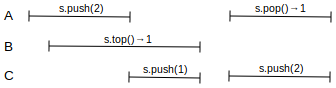
\includegraphics[scale=0.6]{Timeline1.png}
                        \captionsetup{labelformat=empty}
                        \caption{(i)}
                    \end{subfigure}%
                    \begin{subfigure}{.5\textwidth}
                        \centering
                        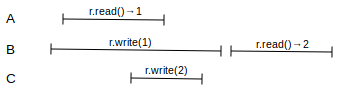
\includegraphics[scale=0.6]{Timeline2.png}
                        \captionsetup{labelformat=empty}
                        \caption{(ii)}
                    \end{subfigure}
                \end{figure}
                \begin{figure}[H]
                    \centering
                    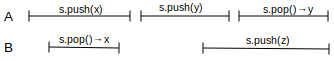
\includegraphics[scale=0.6]{Timeline3.png}
                    \captionsetup{labelformat=empty}
                    \caption{(iii)}
                \end{figure}
            \Question
                \begin{enumerate}[label=(\roman*)]
                    \item We can order this history as
                        \begin{center}
                            \texttt{s.push(2)$\rightarrow$s.push(1)$\rightarrow$s.top():1$\rightarrow$s.pop():1$\rightarrow$s.push(2)}
                        \end{center}
                        We see that this ordering preserves the precedence relationships and describes a legal sequential history. Therefore, this history is linearizable and thereby also sequentially consistent.
                    \item We can order this history as
                        \begin{center}
                            \texttt{r.write(1)$\rightarrow$r.read():1$\rightarrow$r.write(2)$\rightarrow$r.read():2}
                        \end{center}
                        We see that this ordering preserves the precedence relationships and describes a legal sequential history. Therefore, this history is linearizable and thereby also sequentially consistent.
                    \item We can order this history as
                        \begin{center}
                            \texttt{s.push(x)$\rightarrow$s.pop():x$\rightarrow$s.push(y)$\rightarrow$s.pop():y$\rightarrow$s.push(z)}
                        \end{center}
                        We see that this ordering preserves the precedence relationships and describes a legal sequential history. Therefore, this history is linearizable and thereby also sequentially consistent.
                \end{enumerate}
            \Question No, it's not. Consider the following execution. It's easy to see that both \textit{q} and \textit{p} are sequentially consistent, yet the execution as a whole is not sequentially consistent.
                \begin{figure}[H]
                    \centering
                    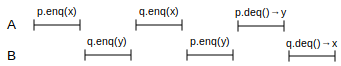
\includegraphics[scale=0.6]{Timeline4.png}
                \end{figure}
            
            
        \Exercise[title={Consensus},label=Cons].\quad \\
            \Question Argue why every n-thread with $n>1$ consensus protocol has a bivalent initial state.
            \Question Which of the following are valid implementations wait-free consensus for the given number N of threads (or an arbitrary number of threads if no N is specified)? Justify your answer.
                \begin{figure}[H]
                    \centering
                    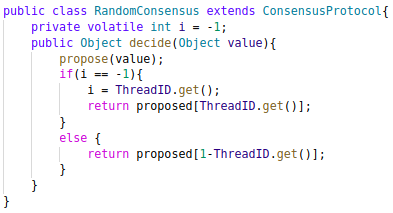
\includegraphics[scale=0.45]{RandomConsensus1.png}
                    \captionsetup{labelformat=empty}
                    \caption{(i) N = 2}
                \end{figure}
                \begin{figure}[H]
                    \centering
                    \begin{subfigure}{.5\textwidth}
                        \centering
                        \vspace{-15pt}
                        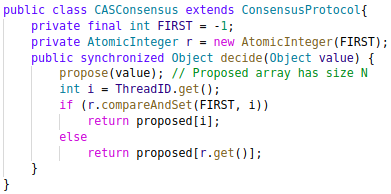
\includegraphics[scale=0.45]{CASConsensus2.png}
                        \captionsetup{labelformat=empty}
                        \caption{(ii)}
                    \end{subfigure}%
                    \begin{subfigure}{.5\textwidth}
                        \centering
                        \vspace{-15pt}
                        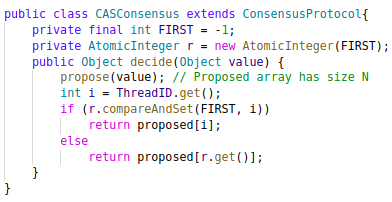
\includegraphics[scale=0.45]{CASConsensus1.png}
                        \captionsetup{labelformat=empty}
                        \caption{(iii)}
                    \end{subfigure}
                \end{figure}
                
        \Answer[ref={Cons}]. \\
            \Question Consider the initial state where \textit{A} has input 0 and \textit{B} has input 1. If \textit{A} finishes the protocol before \textit{B} takes a step, then \textit{A} must decide 0; because a valid consensus protocol must decide some thread's input, and 0 is the only input it has seen. Symmetrically, if \textit{B} finishes the protocol before \textit{A} takes a step, then \textit{B} must decide; because it must decide some thread's input, and 1 is the only input it has seen. It follows that the initial state where \textit{A} has input 0 and \textit{B} has input 1 is bivalent.
            \Question
                \begin{enumerate}[label=(\roman*)]
                    \item Suppose two threads A and B simultaneously see \texttt{i == -1}, i.e. they both enter the if-block, and both have different input values. They will then decide on their own input values, which means the \texttt{decide} method returns two different values, i.e. it's not correct. \\[3mm]
                    We could've also argued that the \texttt{volatile} keyword simply ensures that reads and writes are atomic. As we've shown that atomic registers can't solve two-thread consensus, we would've immediately seen that this protocol can't be correct.
                    \item Note that the \texttt{decide} method is declared as \texttt{synchronized}. We've shown that wait-free implementations can't use locks, this consensus protocol isn't wait-free.
                    \item The threads share an \texttt{AtomicInteger} object, initialized to a constant \texttt{FIRST}, distinct from any thread index. Each thread calls \texttt{compareAndSet} with \texttt{FIRST} as the expected value, and its own index as the new value. If thread \textit{A}'s call returns \texttt{true}, then that method call was first in the linearized order, so \textit{A} decides its own value. Otherwise, \textit{A} reads the current \texttt{AtomicInteger} value, and takes that thread's input from the \texttt{proposed[]} array.
                \end{enumerate}
    \end{ExerciseList}
\pagebreak
\subsection{Solutions}
\shipoutAnswer

\end{document}